\begin{figure}[b!]
	\centering
	\begin{subfigure}[b]{0.49\linewidth}
		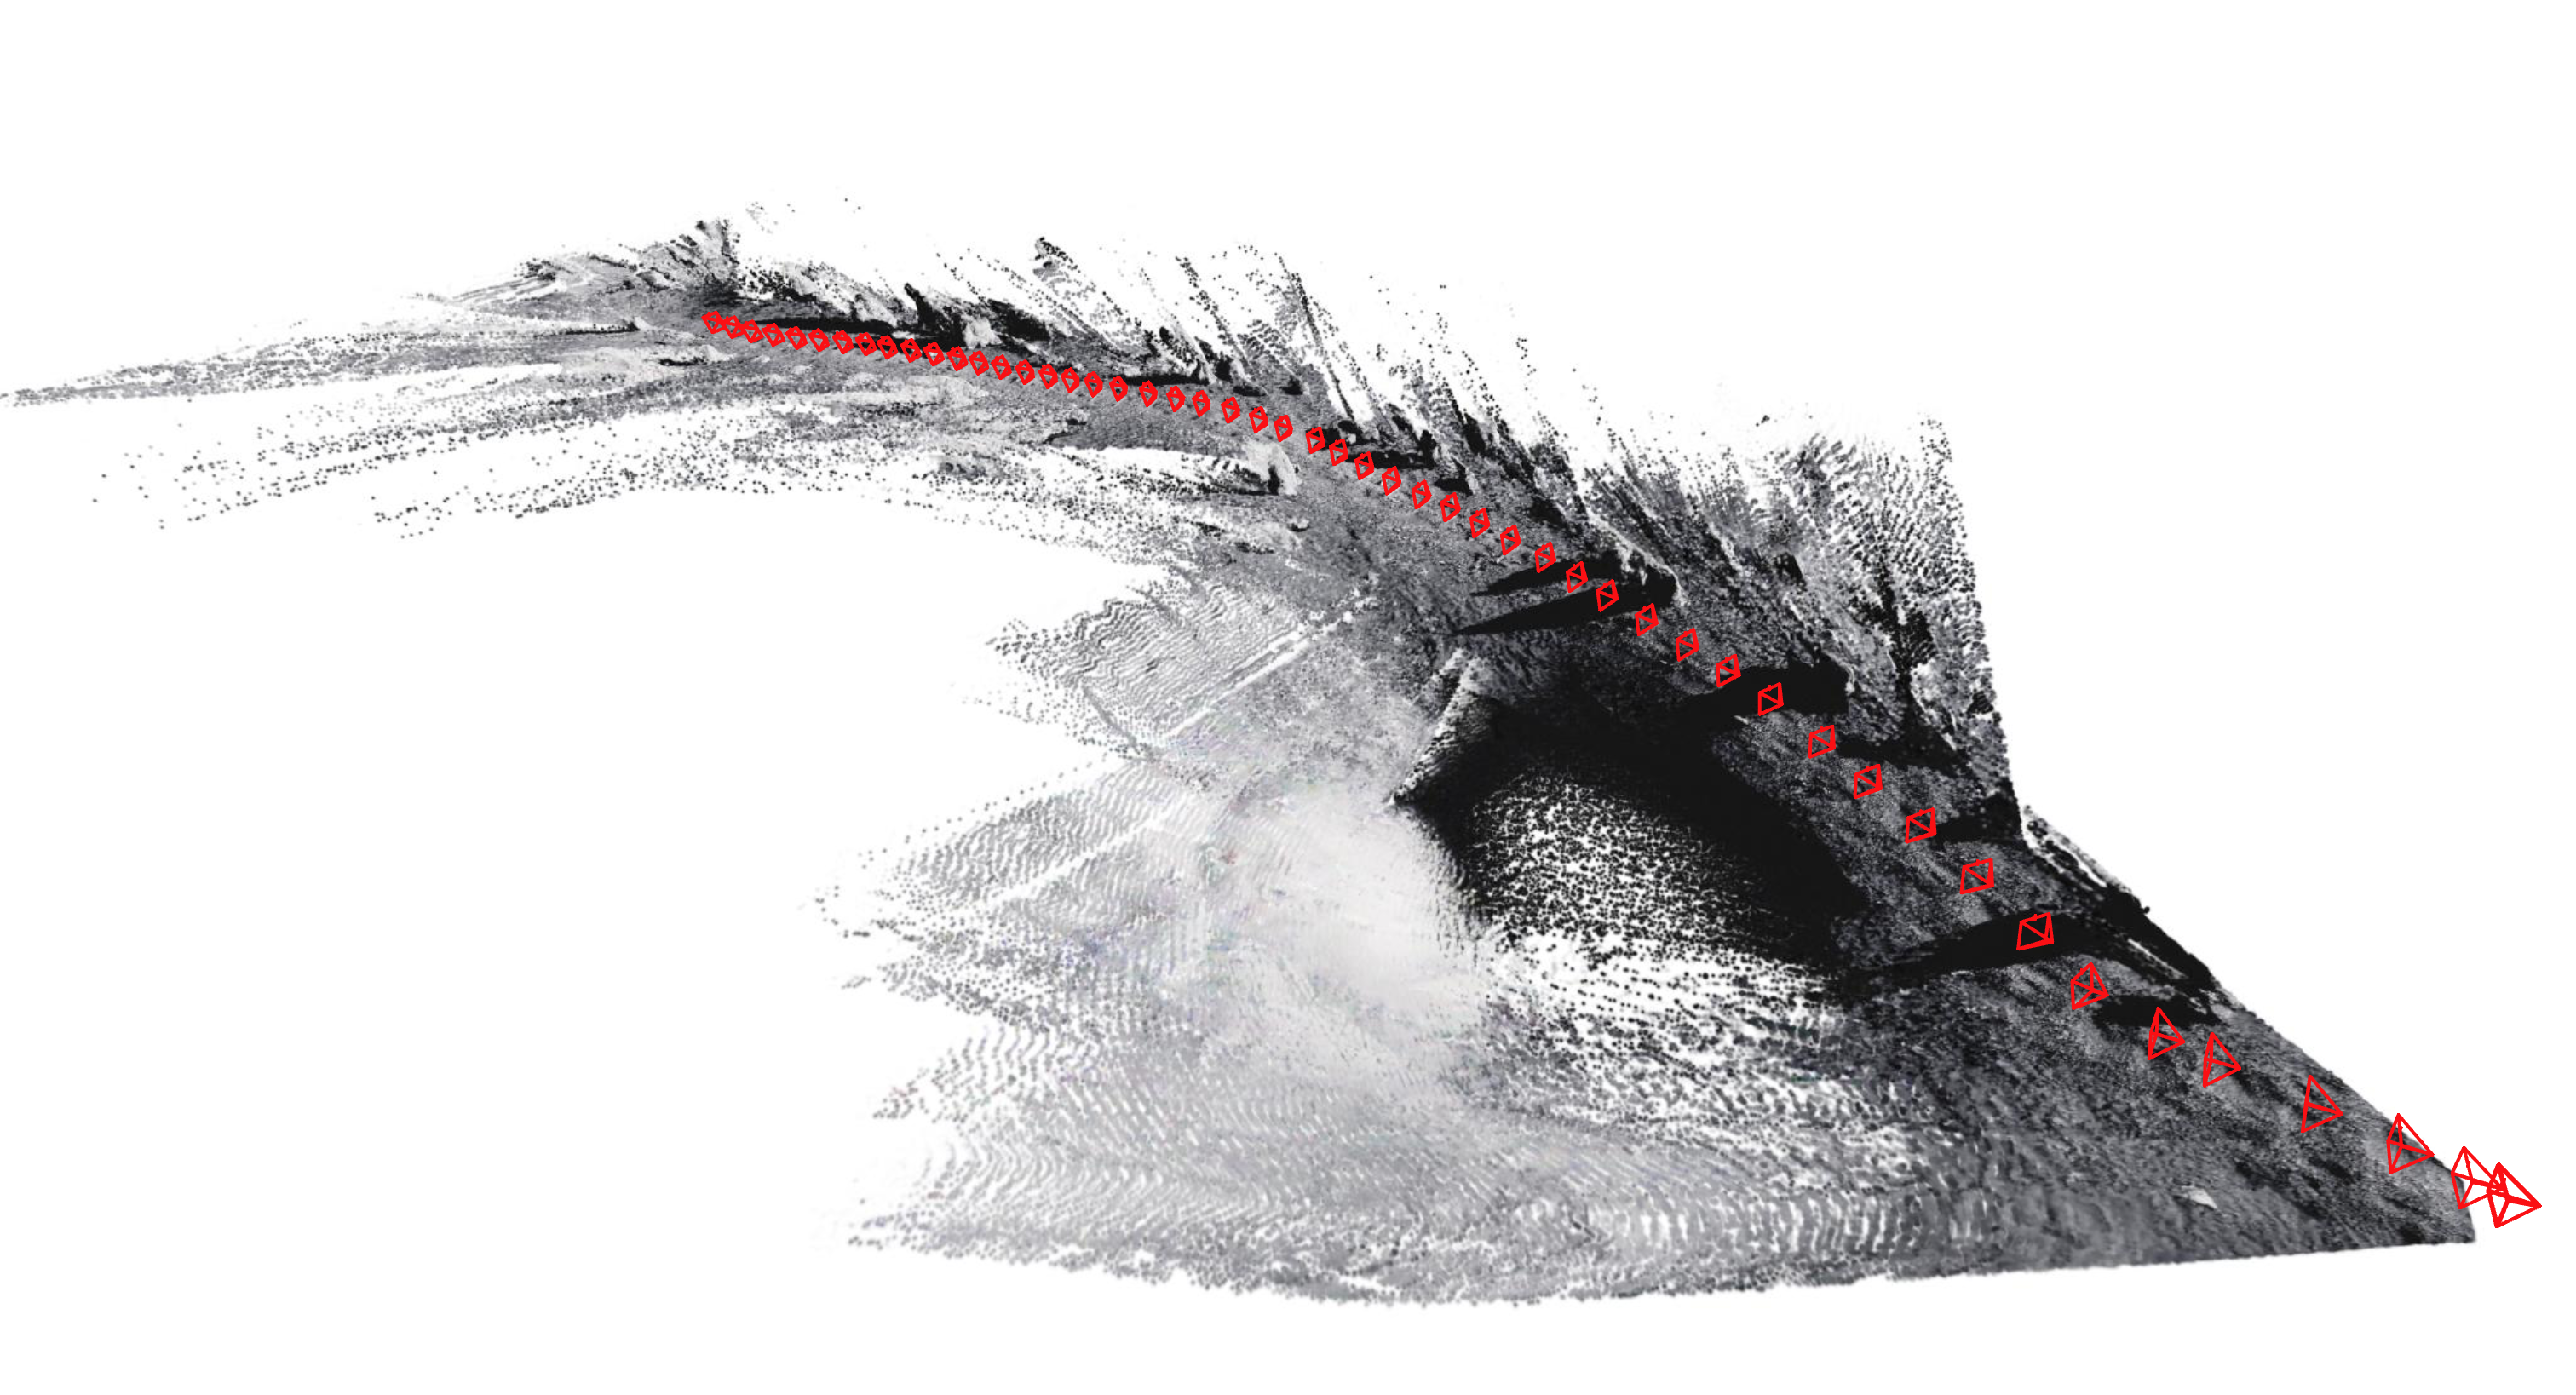
\includegraphics[width=\linewidth]{figures/3dgs/render-partial-rgb.png}
		\caption{\bfseries Initial map (RGB).}
	\end{subfigure}
	\hfill
	\begin{subfigure}[b]{0.49\linewidth}
		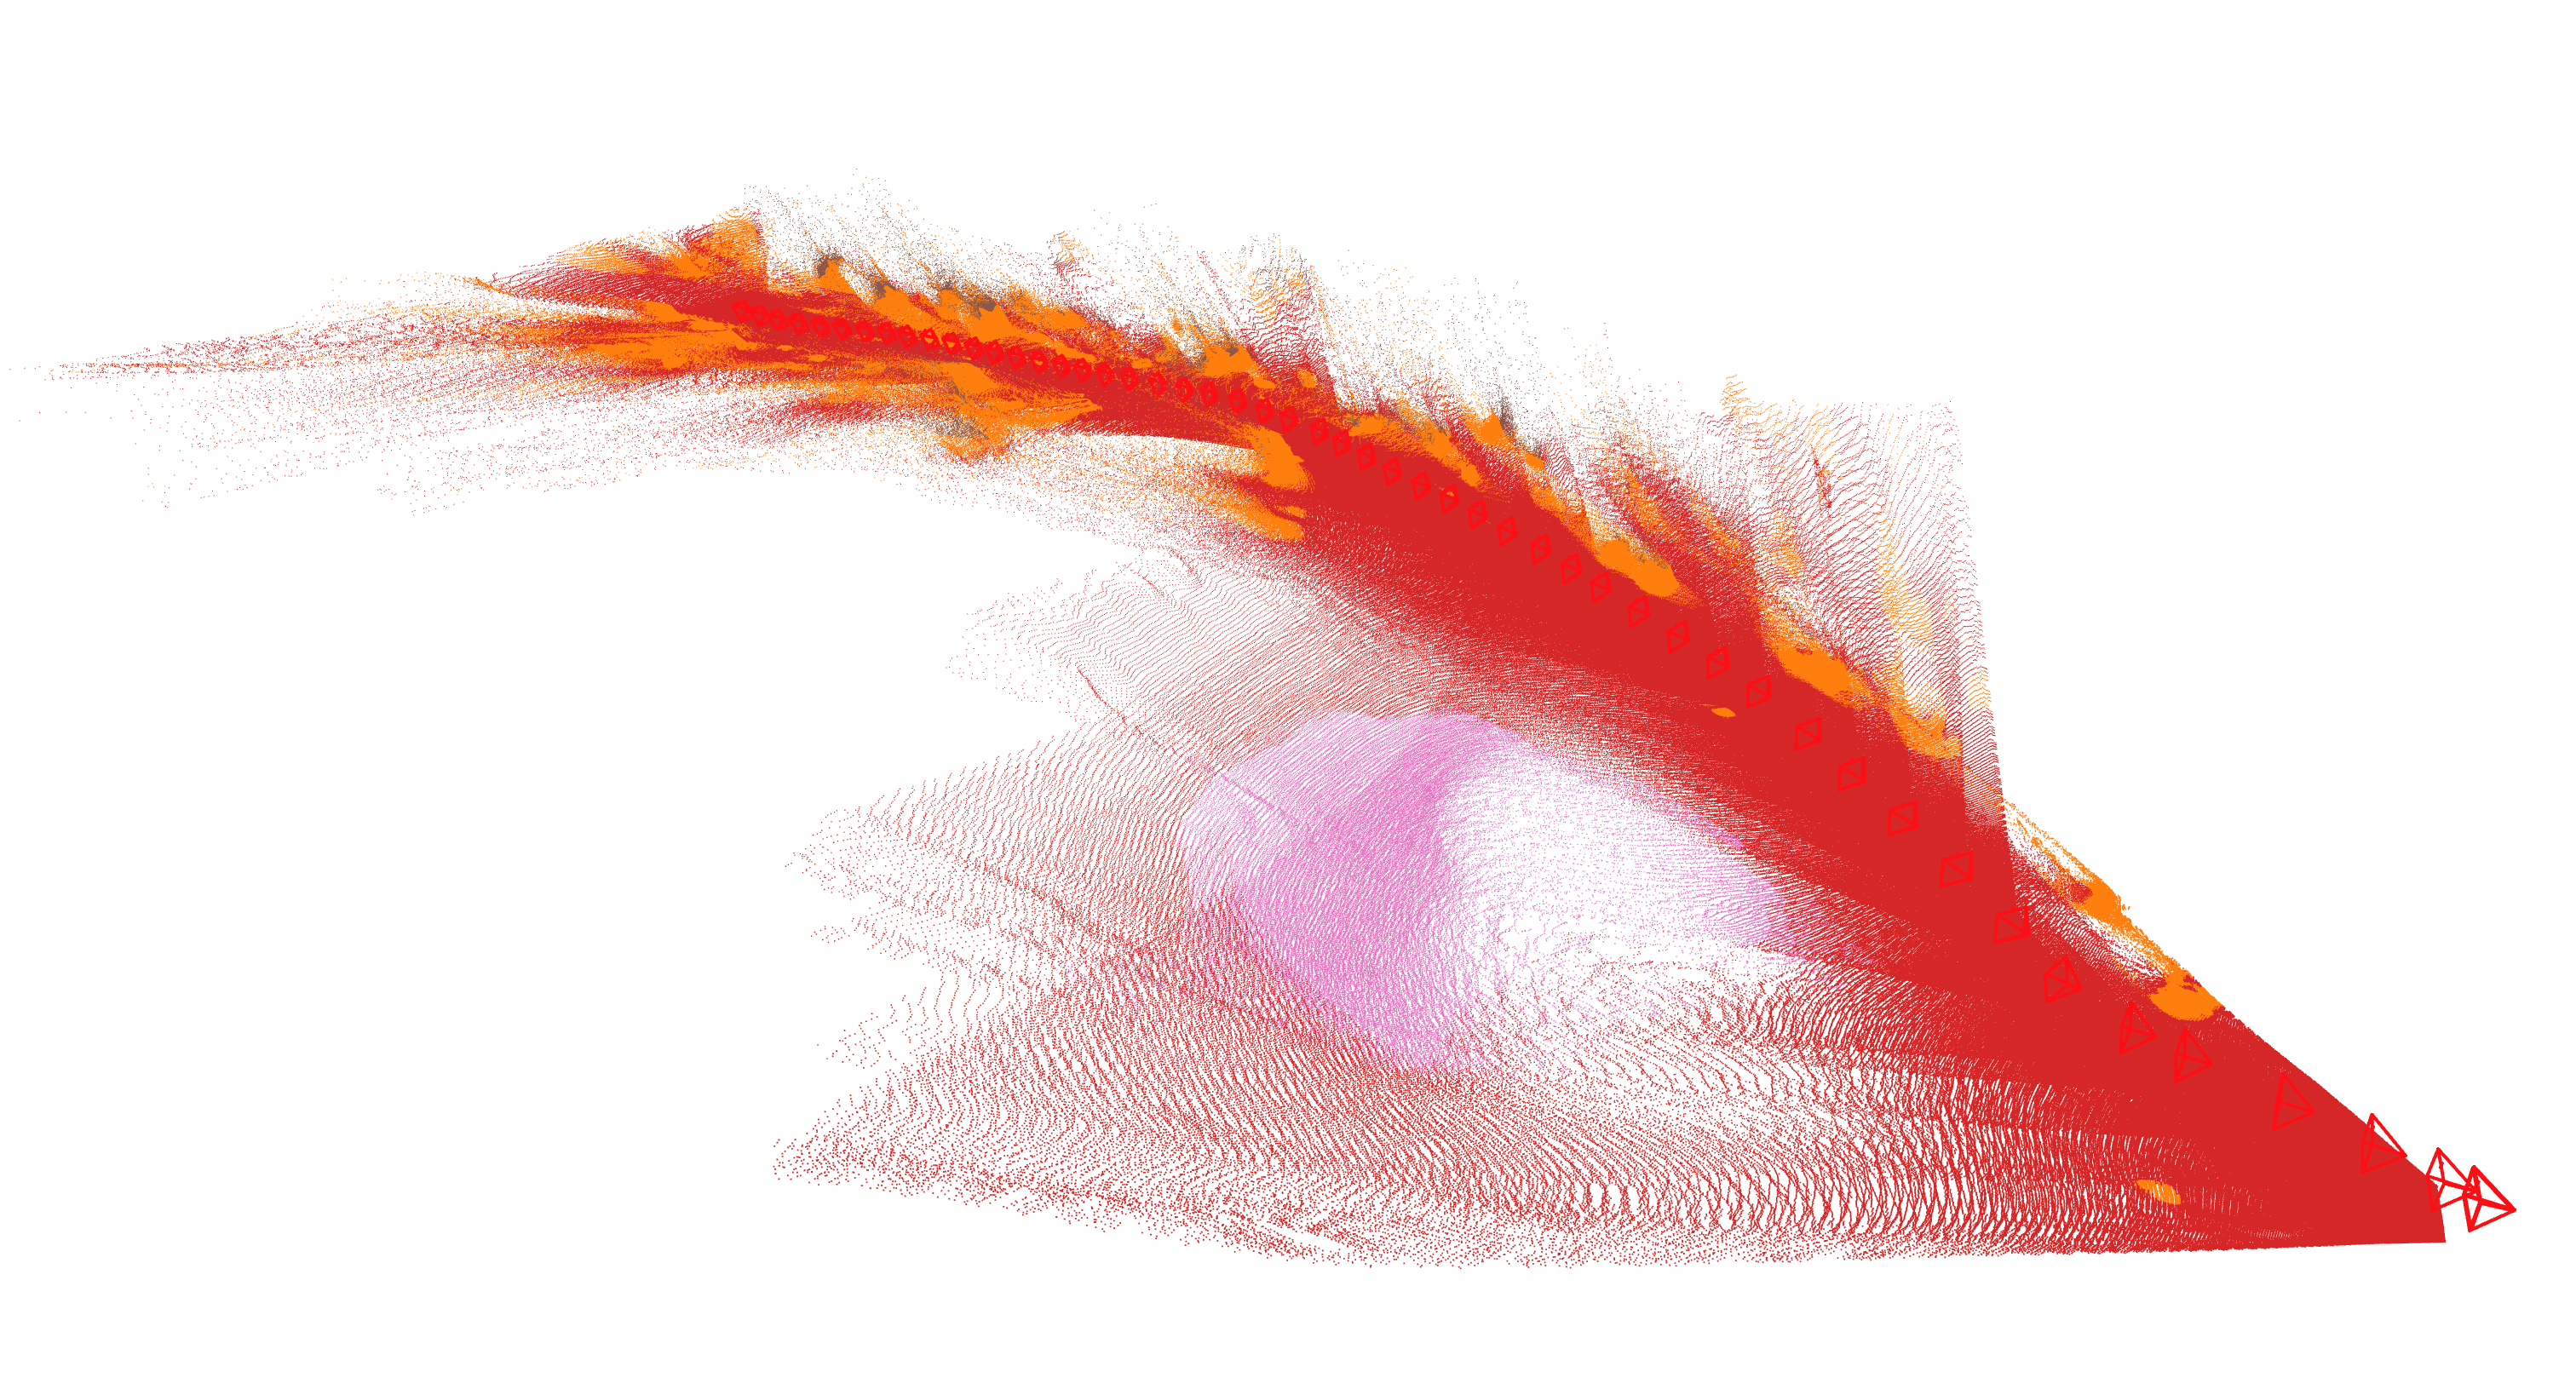
\includegraphics[width=\linewidth]{figures/3dgs/render-partial-semantic.png}
		\caption{\bfseries Partial map (semantic).}
	\end{subfigure}
	\begin{subfigure}[b]{\linewidth}
		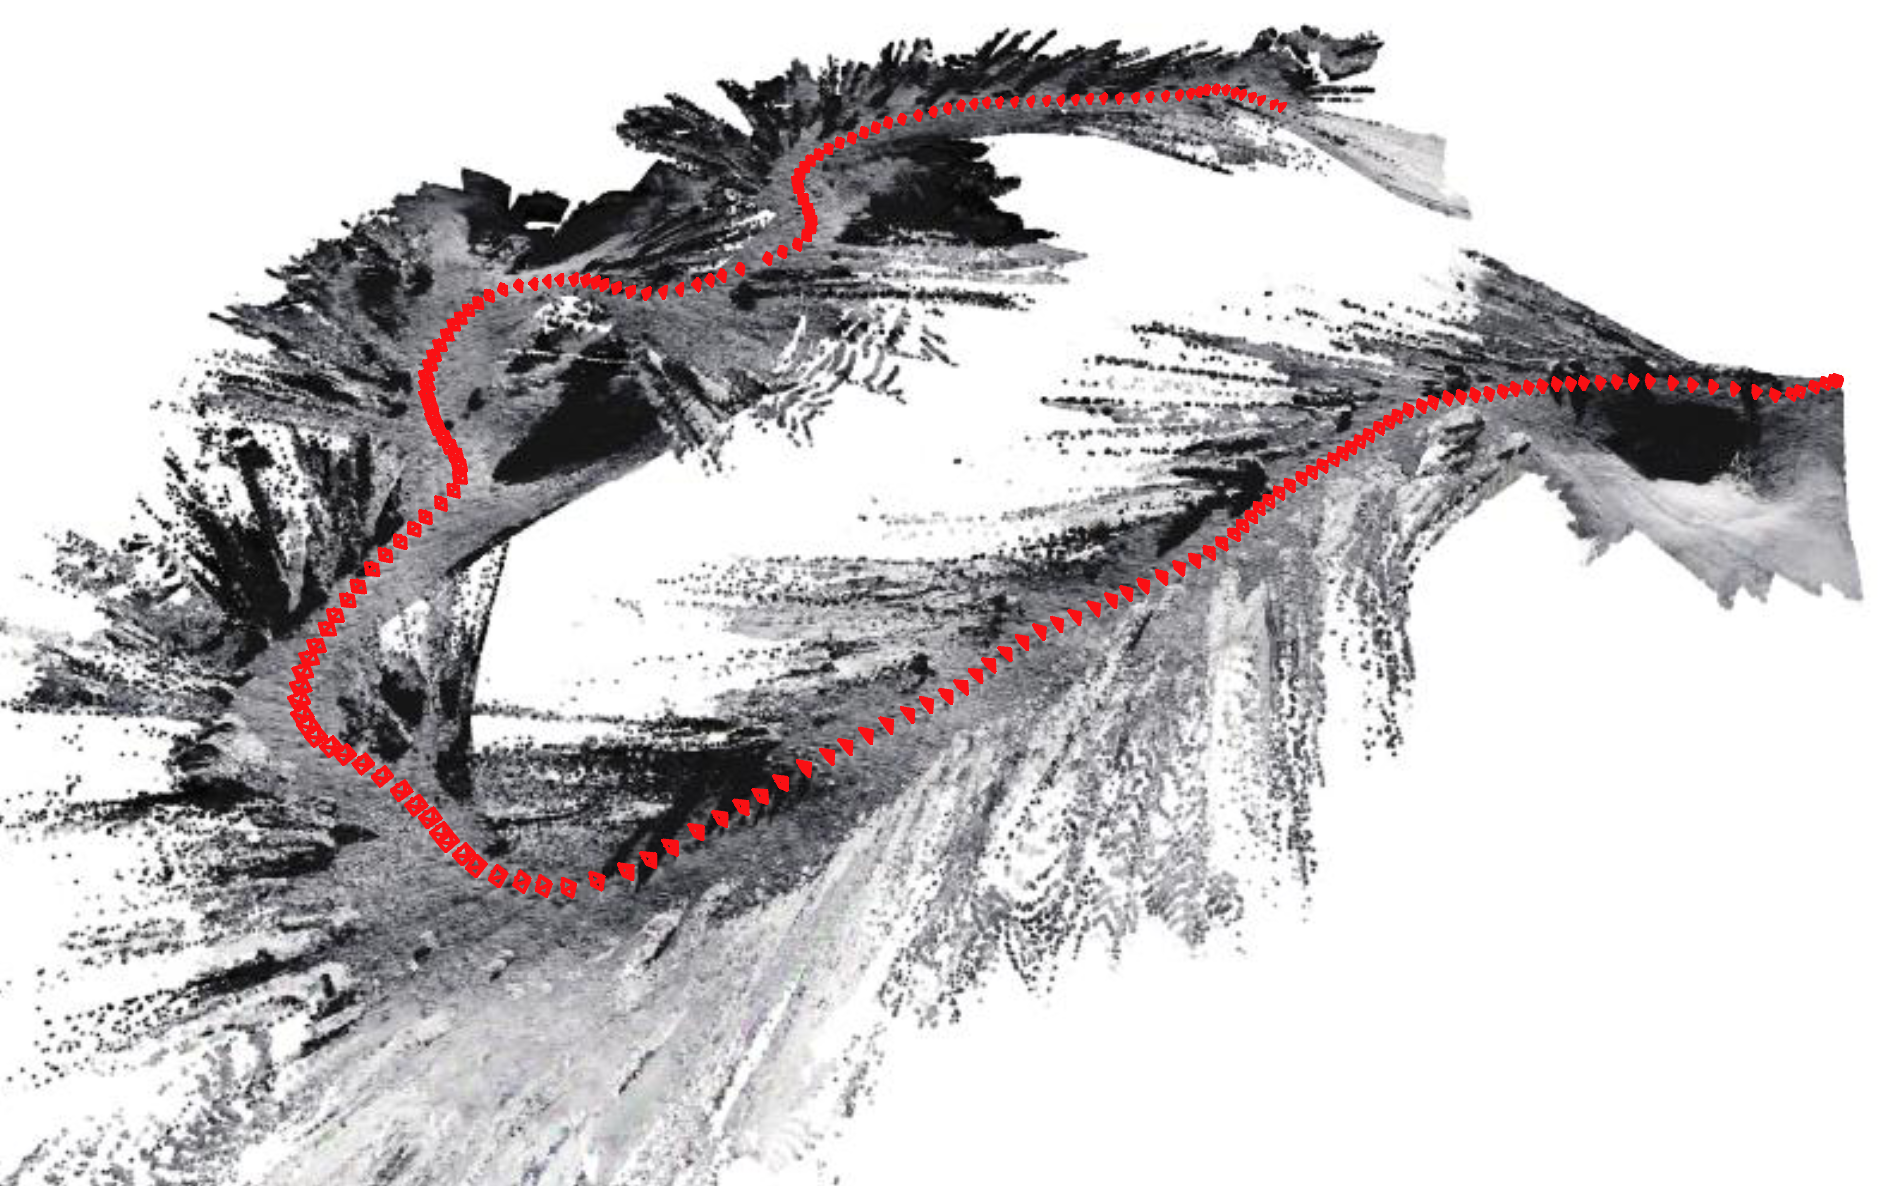
\includegraphics[width=\linewidth,trim=0 0 0 0,clip]{figures/3dgs/render-full.png}
		\caption{\bfseries Final map (RGB).}
	\end{subfigure}
	\caption{\bfseries Partial and final 3DGS maps.}
	\label{fig:map_3dgs}
\end{figure}

\begin{figure*}[t]
	\centering
	\begin{subfigure}[b]{0.3\linewidth}
		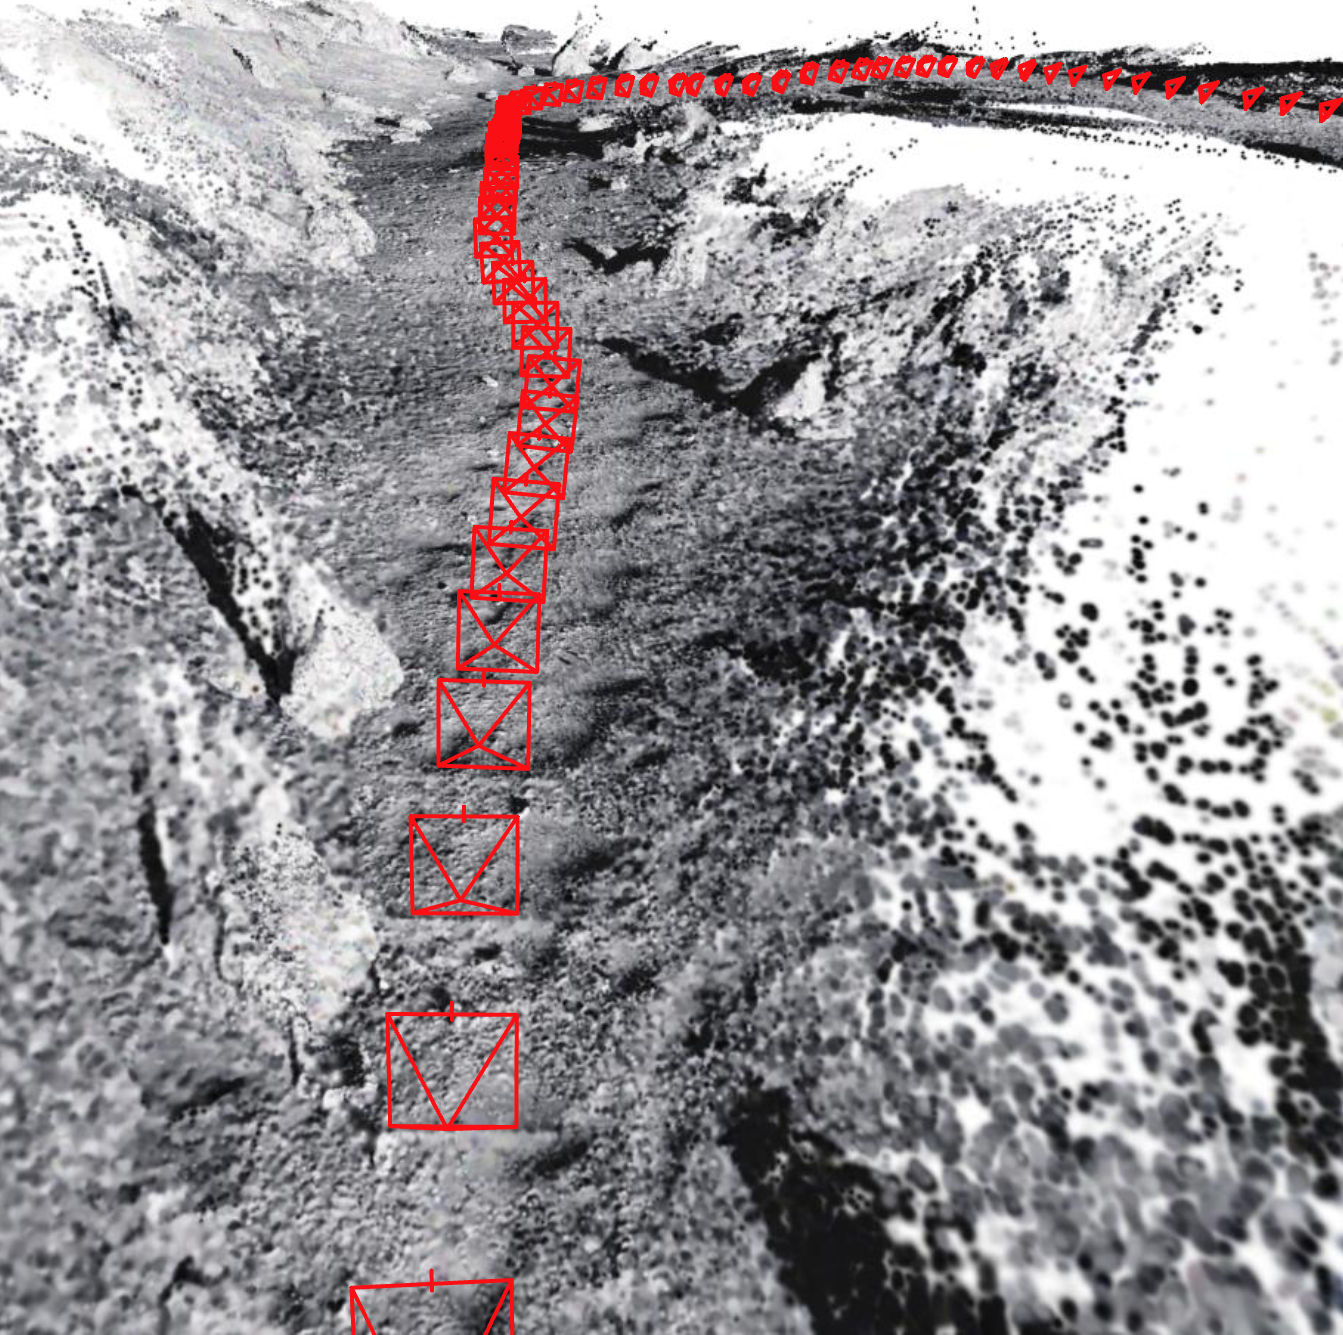
\includegraphics[width=\linewidth]{figures/3dgs/render-birdseye.png}
	\end{subfigure}
	\hfill
	\begin{subfigure}[b]{0.3\linewidth}
		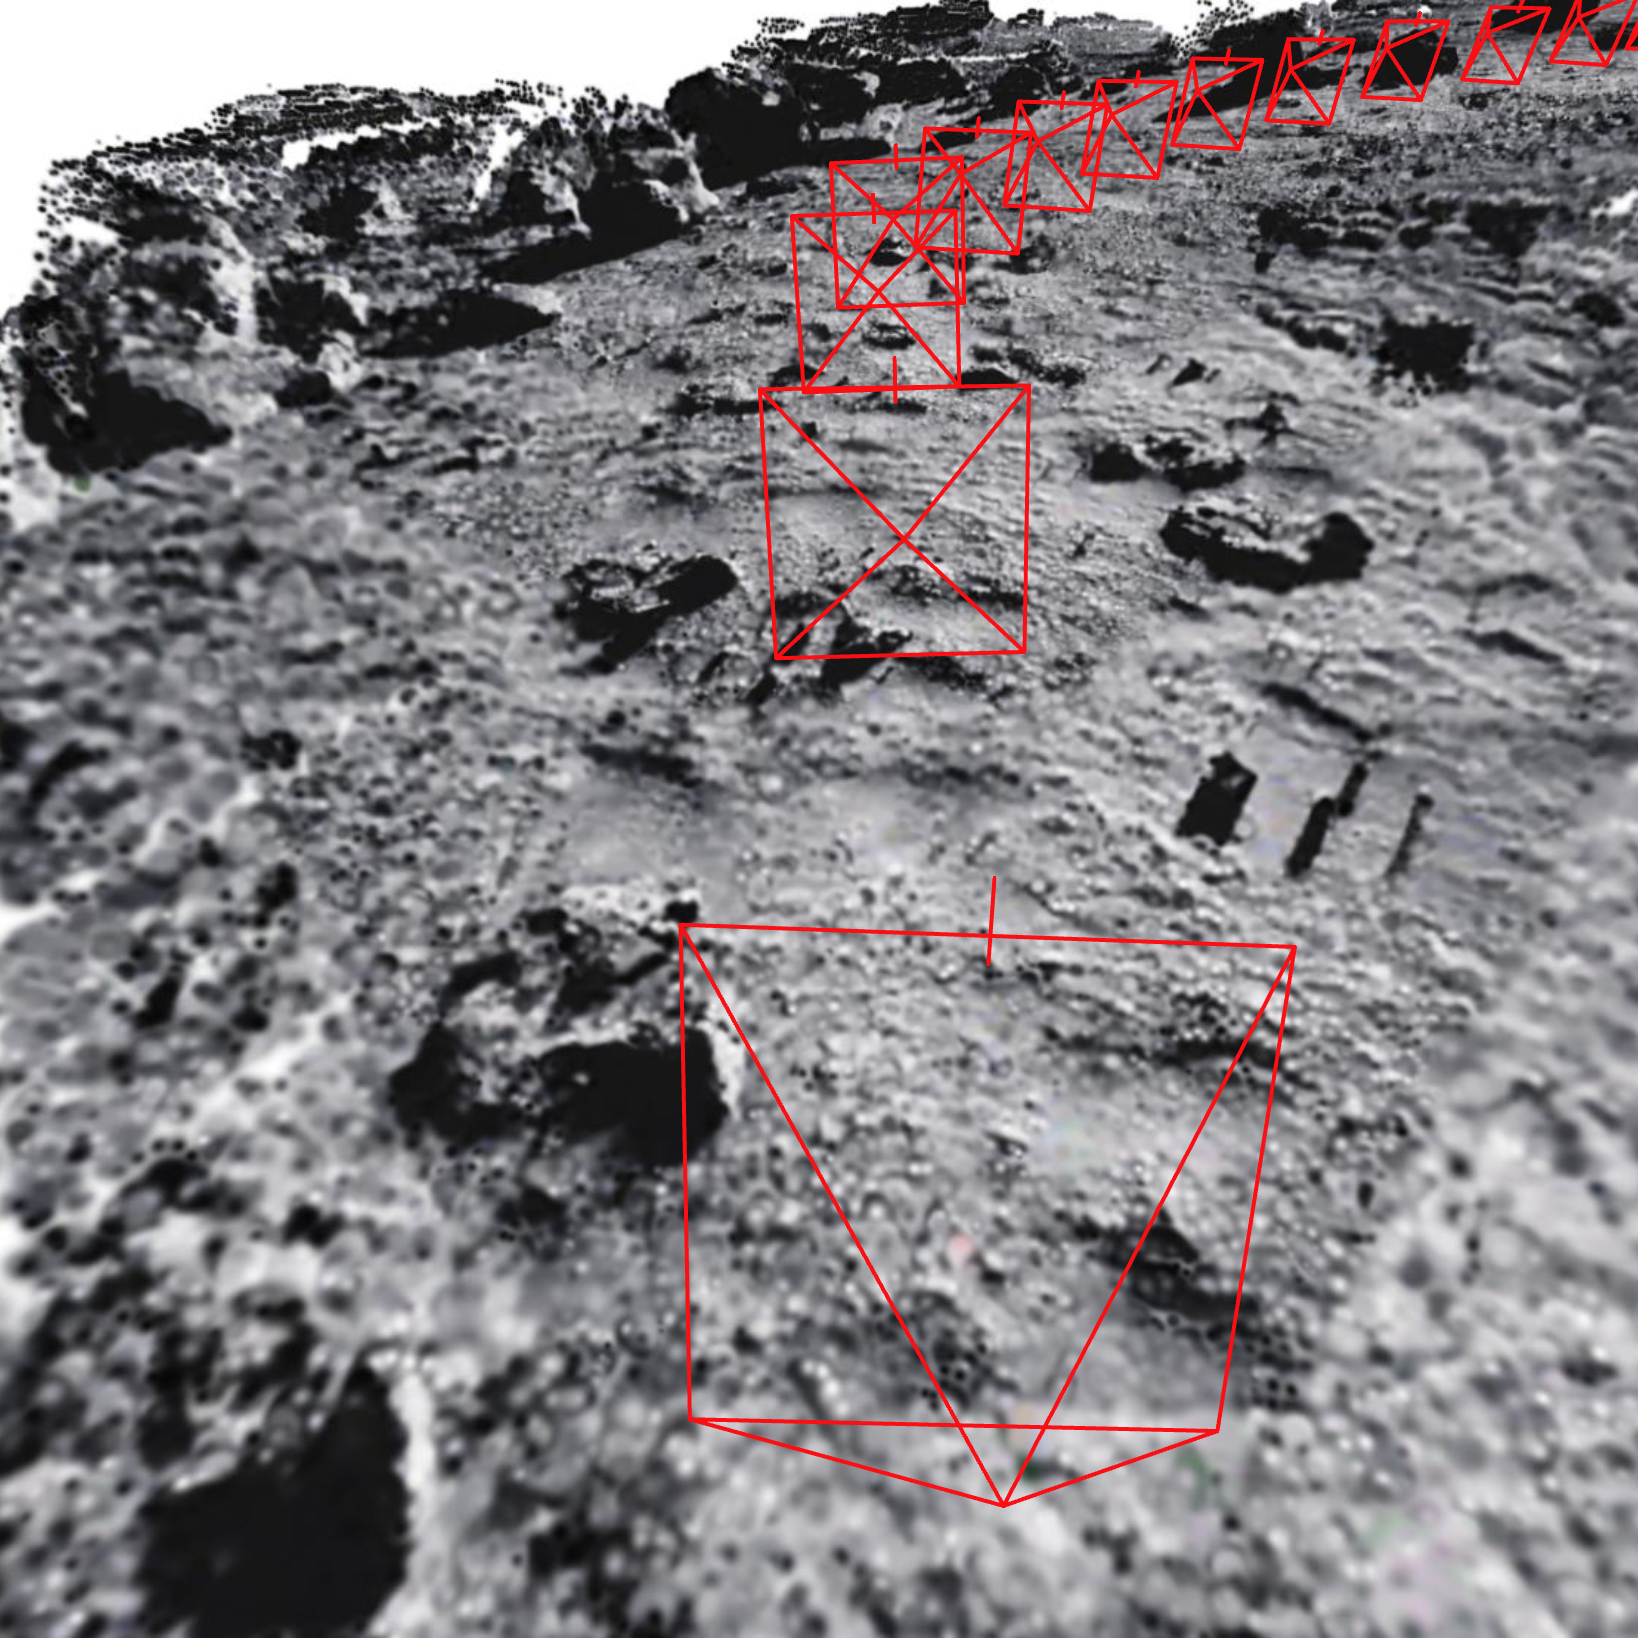
\includegraphics[width=\linewidth,trim=10em 0 0 0,clip]{figures/3dgs/render-close.png}
	\end{subfigure}
	\hfill
	\begin{subfigure}[b]{0.3\linewidth}
		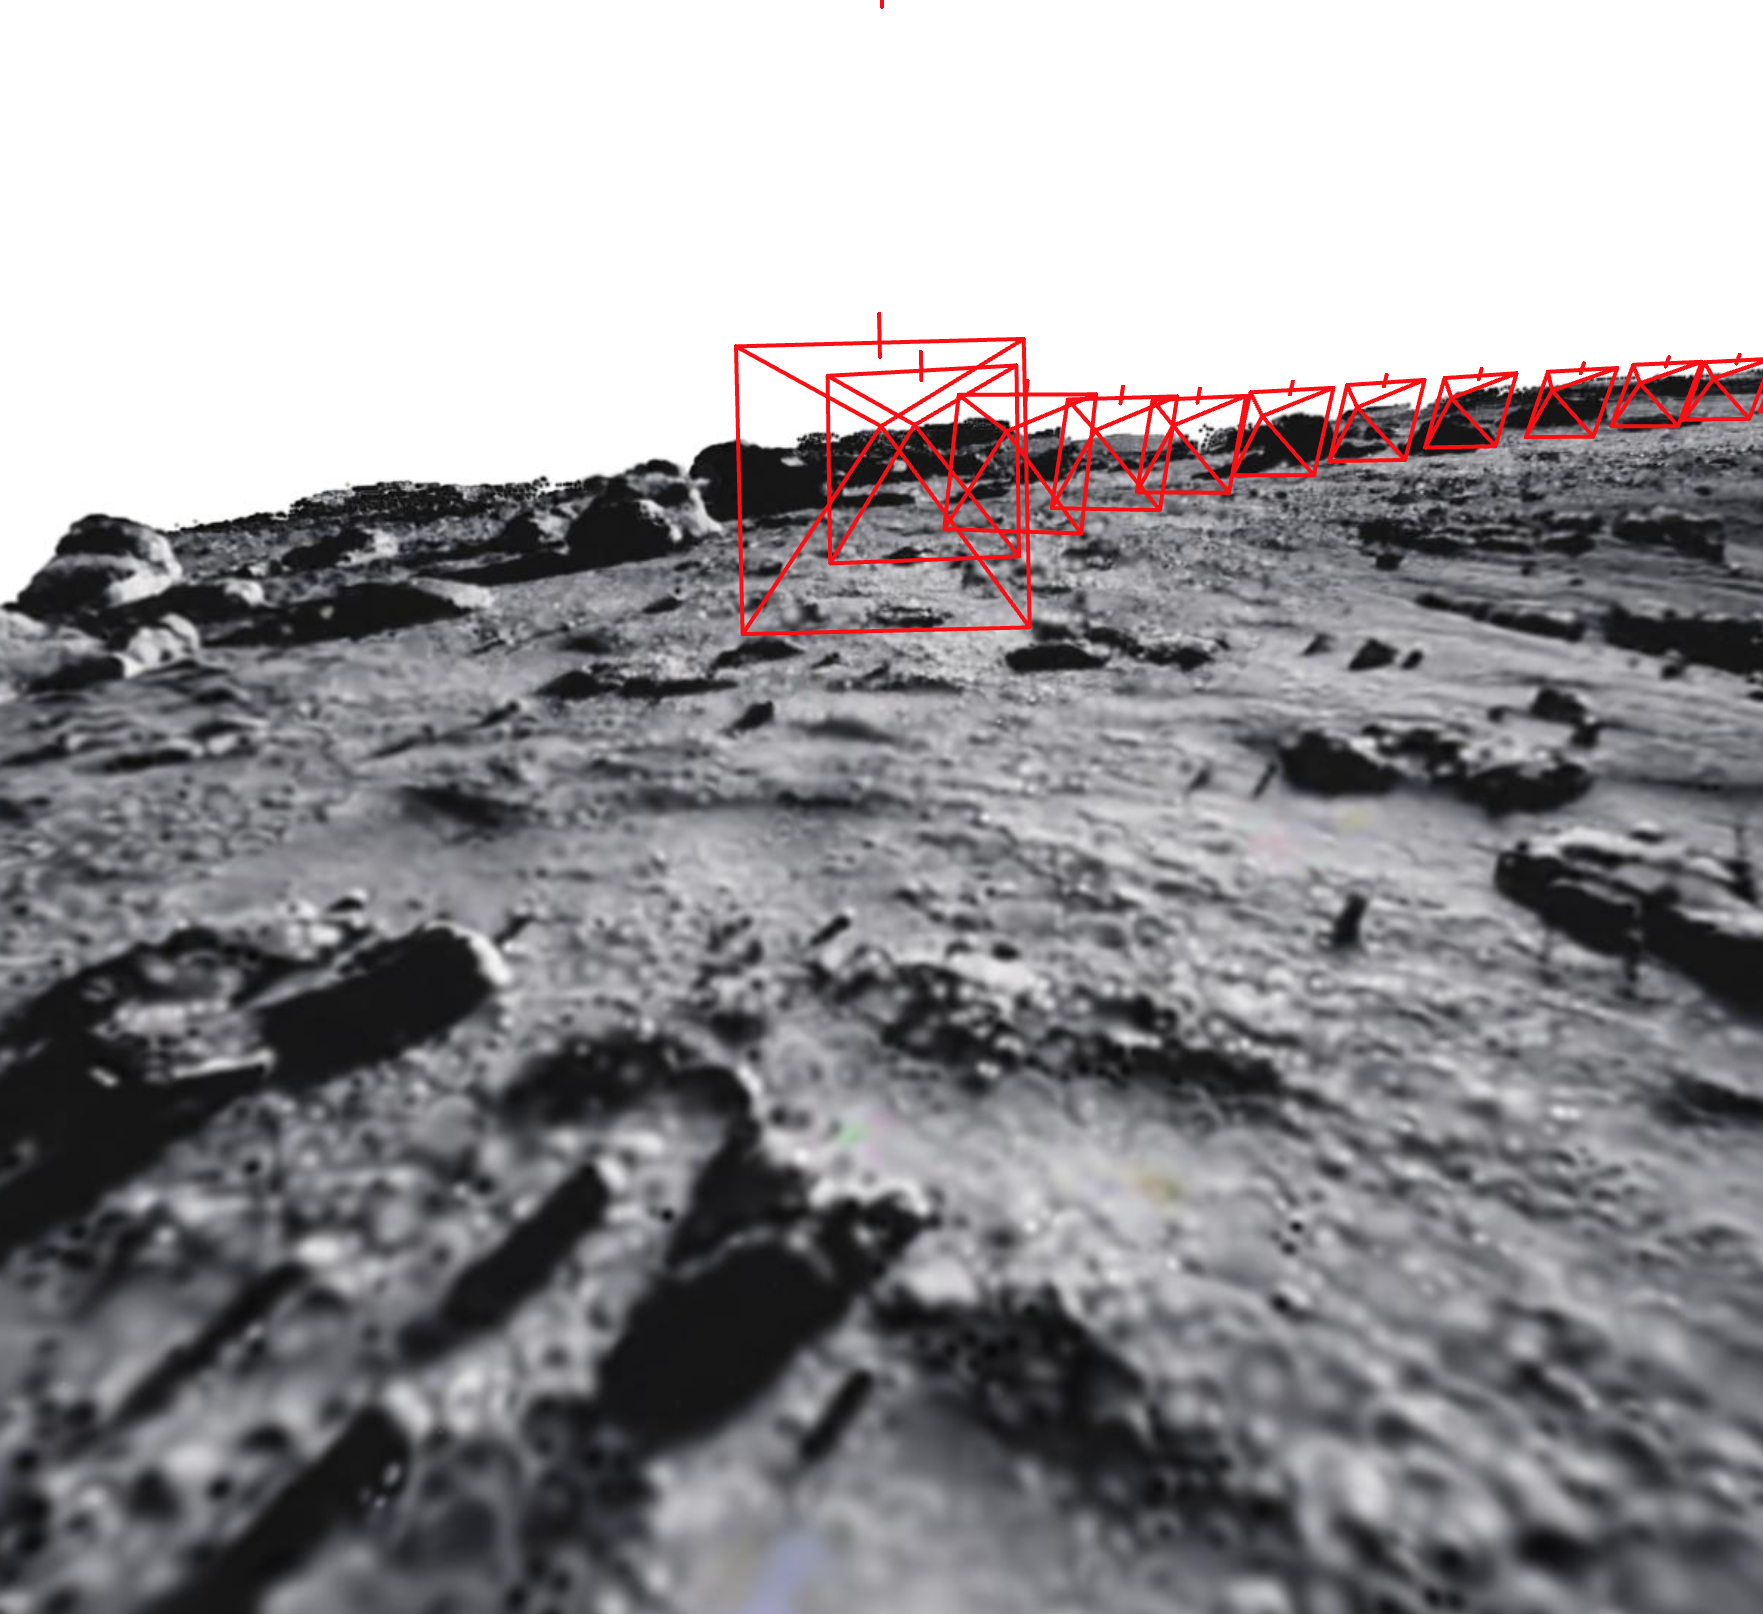
\includegraphics[width=\linewidth]{figures/3dgs/render-camera.png}
	\end{subfigure}
	\caption{\bfseries Qualitative novel view synthesis results rendered from the 3DGS map.}
	\label{fig:novel_views}
\end{figure*}

\begin{table*}[h]
	\centering
	\small
	\caption{\bfseries Summary of surface reconstruction results. Precision and recall using a threshold of 10 cm.}
	\label{tab:surface_reconstruction_short}
	\begin{tabular}[t]{|lrrrrrr|}
		\hline
		\multirow{2}{*}{\textbf{Metric}}               &
		\multicolumn{1}{c}{\textbf{Accuracy}}          &
		\multicolumn{1}{c}{\textbf{Completion}}        &
		\multicolumn{1}{c}{\textbf{Precision}}         &
		\multicolumn{1}{c}{\textbf{Recall}}            &
		\multicolumn{1}{c}{\textbf{F-Score}}           &
		\multicolumn{1}{c|}{\textbf{Height Error}}
		\\
		\multicolumn{1}{|c}{}                          &
		\multicolumn{1}{c}{\textbf{[cm] $\downarrow$}} &
		\multicolumn{1}{c}{\textbf{[cm] $\downarrow$}} &
		\multicolumn{1}{c}{\textbf{[\%] $\uparrow$}}   &
		\multicolumn{1}{c}{\textbf{[\%] $\uparrow$}}   &
		\multicolumn{1}{c}{\textbf{[\%] $\uparrow$}}   &
		\multicolumn{1}{c|}{\textbf{[cm] $\downarrow$}}                                          \\
		\hline\hline
		3DGS                                           & 19.4 & 25.8 & 73.1 & 78.9 & 75.9 & 10.8 \\
		+ GT Segmentation                              & 19.4 & 25.8 & 73.1 & 78.8 & 75.9 & 10.8 \\
		+ GT Depth                                     & 13.3 & 29.4 & 82.3 & 81.1 & 81.7 & 6.0  \\
		+ GT Depth + GT Segmentation                   & 13.3 & 29.4 & 82.3 & 81.1 & 81.7 & 6.0  \\
		\hline
		Point Cloud                                    & 19.2 & 26.0 & 77.1 & 78.0 & 77.5 & 9.8  \\
		+ GT Segmentation                              & 19.2 & 26.0 & 77.1 & 78.0 & 77.5 & 9.8  \\
		+ GT Depth                                     & 12.5 & 29.8 & 89.5 & 81.0 & 85.1 & 4.2  \\
		+ GT Depth + GT Segmentation                   & 12.5 & 29.8 & 89.5 & 81.0 & 85.1 & 4.2  \\
		\hline
	\end{tabular}
\end{table*}

\subsection{Surface Reconstruction}
% Intro
We evaluate our real-time mapping framework on a 500-meter traverse within a scene from the LuSNAR dataset. The input is sourced from a single front-facing stereo camera pair (512x512 pixel resolution) at a rate of 1 Hz. The pipeline uses U-Net++ for semantic segmentation and RAFT-Stereo for dense depth estimation.
We use a ground truth map sampled of 1 cm resolution.
To benchmark our method and selection of perception models, we compare the reconstruction accuracy of this full pipeline against a configuration that uses ground truth depth and segmentation. For this evaluation, we assume ground truth poses are provided, as our primary focus is to analyze the mapping feasibility and performance independent of a front-end tracking system.

% Note on surface reconstruction metrics
For this preliminary analysis, it is important to note how the surface reconstruction metrics are computed. We extract a point cloud from the 3DGS map by using only the position of each Gaussian. This approach is a simplification, as the center of a Gaussian is not constrained to lie directly on the physical surface. By treating the Gaussians as discrete points, we do not yet leverage the continuous, density-based surface representation that is a key advantage of the method~\cite{wolf_gs2mesh_2025}. We are currently developing a more accurate surface reconstruction pipeline that will use this density information to provide a better evaluation of the map's quality.

% Qualitative results
\Cref{fig:map_3dgs} shows the output of the mapping process, displaying a partial 3DGS map that visualizes the semantic information embedded within each Gaussian, as well as the final, complete map for the entire traverse. The quality of the scene representation is further demonstrated in \Cref{fig:novel_views}, which presents novel view synthesis results. These images are rendered from viewpoints that were not seen during the mapping process, highlighting the framework's ability to build a coherent and renderable 3D model of the environment.

% Quantitative results
The quantitative results for the map reconstruction are presented in \Cref{tab:surface_reconstruction,tab:surface_reconstruction_short}. The first table provides a detailed breakdown of performance for each semantic class, while the second summarizes the average results across all classes. From these aggregate results, our full pipeline achieves a mean height error of 10 cm. With a 10 cm evaluation threshold, the precision and recall metrics are over 70\%, indicating that the majority of the reconstructed surface is geometrically consistent with the ground truth.

A key finding is the minimal impact of the segmentation model's accuracy on the final geometry; using ground truth semantic labels resulted in negligible changes to the aggregate metrics, demonstrating the high performance of the U-Net++ model. The per-class breakdown in \Cref{tab:surface_reconstruction} reveals that reconstruction errors are largest for the crater category. This is an expected outcome, as craters in the trajectory are typically distant from the rover and are often poorly illuminated within deep shadows, making accurate depth estimation challenging.
A qualitative analysis of the reconstruction shows that the largest geometric errors are concentrated along the dark, high-contrast edges of rocks. These regions represent a common failure mode for both the depth estimation and semantic segmentation models, which struggle to distinguish shadowed rock boundaries from the dark sky or shadowed regolith.

When using estimated depth under ideal pose conditions, the 3DGS pipeline's performance is quantitatively similar to the point cloud baseline, with the cm-level difference in average height error falling close to the 1 cm resolution of the ground truth map. Our next analysis will explore more challenging scenarios, such as re-mapping the same area to evaluate consistency or introducing pose noise. We hypothesize that in such cases, the 3DGS framework's ability to jointly optimize both the map and camera poses to achieve multi-view consistency would demonstrate a significant advantage.

% Memory usage
\Cref{tab:memory_usage_3dgs} and \Cref{tab:memory_usage_point_cloud} show the memory requirements for the 500-meter traverse, resulting in a map of approximately 15 million Gaussians and 12 million points. It is important to note that the current memory usage can be significantly reduced, as techniques for pruning and compressing the 3DGS map, keyframe buffer, and baseline point cloud are left as future work~\cite{bagdasarian_3dgszip_2025}. The 3DGS map representation itself (775 MB) is more compact than the sum of the images taken RGB (2x1200 MB), indicating that the 3DGS map can become a memory efficient alternative that offers rendering capabilities.

Compared to a traditional semantic point cloud of similar scale, the 3DGS map requires about 2.5 times more memory (336 MB for the point cloud). However, the memory footprint of our framework is highly dependent on the configuration. Only a small subset of the keyframe buffer storing RGB images, depths, and masks is necessary for global optimization tasks like loop closure or refining past poses.
Similarly, the memory for strategy variables is only required for visible Gaussians and can be pruned for areas of the map no longer in view, substantially reducing the active memory load.
Further analysis and optimization of the framework's memory and computational requirements is an area of ongoing work. We are investigating compression techniques for both the 3D Gaussian representation and the keyframe buffer to substantially reduce the memory footprint for long-range traverses.



\begin{table*}[h]
	\centering
	\small
	\begin{minipage}[t]{0.68\linewidth}
		\centering
		\caption{3DGS memory usage.}
		\label{tab:memory_usage_3dgs}
		\centering
		\begin{tabular}[t]{|lrlr|lr|}
			\hline
			\textbf{GPU VRAM} &        &                   & 995 MB & \textbf{System RAM} & 1900 MB \\
			\hline\hline
			\textbf{3DGS}     & 830 MB & \textbf{Strategy} & 165 MB & \textbf{Buffer}     & 1900 MB \\
			~~Rotations       & 222 MB & ~~Radii           & 55 MB  & ~~RGBs              & 1200 MB \\
			~~Means           & 166 MB & ~~Gradients       & 55 MB  & ~~Depths            & 400 MB  \\
			~~Scales          & 166 MB & ~~Counts          & 55 MB  & ~~Masks             & 200 MB  \\
			~~Features        & 166 MB &                   &        & ~~Labels            & 100 MB  \\
			~~Opacities       & 55 MB  &                   &        &                     &         \\
			~~Labels          & 55 MB  &                   &        &                     &         \\
			\hline
		\end{tabular}
	\end{minipage}%
	\begin{minipage}[t]{0.3\linewidth}
		\centering
		\caption{Point Cloud memory usage.}
		\label{tab:memory_usage_point_cloud}
		\begin{tabular}[t]{|lr|}
			\hline
			\textbf{System RAM} & 336 MB \\\hline\hline
			~~Points            & 144 MB \\
			~~Color             & 144 MB \\
			~~Label             & 48 MB  \\\hline
		\end{tabular}
	\end{minipage}
\end{table*}



\begin{table*}[h]
	\centering
	\small
	\caption{\bfseries Surface reconstruction results. Precision and recall using a threshold of 10 cm.}
	\label{tab:surface_reconstruction}
	\begin{tabular}[t]{|lrrrrrr|}
		\hline
		\multirow{2}{*}{\textbf{Metric}}               &
		\multicolumn{1}{c}{\textbf{Accuracy}}          &
		\multicolumn{1}{c}{\textbf{Completion}}        &
		\multicolumn{1}{c}{\textbf{Precision}}         &
		\multicolumn{1}{c}{\textbf{Recall}}            &
		\multicolumn{1}{c}{\textbf{F-Score}}           &
		\multicolumn{1}{c|}{\textbf{Height Error}}
		\\
		\multicolumn{1}{|c}{}                          &
		\multicolumn{1}{c}{\textbf{[cm] $\downarrow$}} &
		\multicolumn{1}{c}{\textbf{[cm] $\downarrow$}} &
		\multicolumn{1}{c}{\textbf{[\%] $\uparrow$}}   &
		\multicolumn{1}{c}{\textbf{[\%] $\uparrow$}}   &
		\multicolumn{1}{c}{\textbf{[\%] $\uparrow$}}   &
		\multicolumn{1}{c|}{\textbf{[cm] $\downarrow$}}                                           \\ \hline\hline
		\multicolumn{7}{|l|}{\textbf{3DGS}}                                                       \\ \hline
		Rock                                           & 64.6  & 27.0 & 22.9 & 56.9 & 32.6 & 16.2 \\
		Regolith                                       & 14.5  & 28.0 & 81.8 & 82.0 & 81.9 & 8.5  \\
		Crater                                         & 944.7 & 27.1 & 13.2 & 41.5 & 20.0 & 75.3 \\
		All                                            & 19.4  & 25.8 & 73.1 & 78.9 & 75.9 & 10.8 \\
		\hline
		\multicolumn{7}{|l|}{\textbf{+ GT Segmentation}}                                          \\ \hline
		Rock                                           & 64.7  & 26.5 & 23.0 & 56.8 & 32.7 & 16.3 \\
		Regolith                                       & 14.4  & 28.0 & 81.8 & 82.0 & 81.9 & 8.5  \\
		Crater                                         & 936.2 & 27.6 & 13.4 & 41.4 & 20.2 & 75.1 \\
		All                                            & 19.4  & 25.8 & 73.1 & 78.8 & 75.9 & 10.8 \\
		\hline
		\multicolumn{7}{|l|}{\textbf{+ GT Depth}}                                                 \\ \hline
		Rock                                           & 29.5  & 34.4 & 51.6 & 55.3 & 53.4 & 7.5  \\
		Regolith                                       & 10.2  & 30.0 & 87.3 & 85.2 & 86.2 & 5.3  \\
		Crater                                         & 384.3 & 47.5 & 42.0 & 73.3 & 53.4 & 42.0 \\
		All                                            & 13.3  & 29.4 & 82.3 & 81.1 & 81.7 & 6.0  \\
		\hline
		\multicolumn{7}{|l|}{\textbf{+ GT Depth + GT Segmentation}}                               \\ \hline
		Rock                                           & 27.7  & 35.5 & 52.1 & 55.5 & 53.8 & 7.4  \\
		Regolith                                       & 10.0  & 30.5 & 87.5 & 85.4 & 86.4 & 5.2  \\
		Crater                                         & 344.5 & 48.8 & 43.2 & 73.4 & 54.4 & 40.8 \\
		All                                            & 13.3  & 29.4 & 82.3 & 81.1 & 81.7 & 6.0  \\ \hline\hline
		\multicolumn{7}{|l|}{\textbf{Point Cloud}}                                                \\ \hline
		Rock                                           & 64.3  & 27.9 & 25.7 & 55.2 & 35.1 & 15.9 \\
		Regolith                                       & 13.6  & 28.1 & 87.2 & 81.6 & 84.3 & 7.0  \\
		Crater                                         & 975.5 & 27.1 & 15.1 & 44.9 & 22.6 & 74.7 \\
		All                                            & 19.2  & 26.0 & 77.1 & 78.0 & 77.5 & 9.8  \\
		\hline
		\multicolumn{7}{|l|}{\textbf{+ GT Segmentation}}                                          \\ \hline
		Rock                                           & 64.4  & 27.5 & 25.8 & 55.4 & 35.2 & 16.0 \\
		Regolith                                       & 13.6  & 28.1 & 87.2 & 81.7 & 84.3 & 7.0  \\
		Crater                                         & 967.1 & 27.6 & 15.4 & 44.8 & 22.9 & 74.4 \\
		All                                            & 19.2  & 26.0 & 77.1 & 78.0 & 77.5 & 9.8  \\
		\hline
		\multicolumn{7}{|l|}{\textbf{+ GT Depth}}                                                 \\ \hline
		Rock                                           & 29.9  & 35.9 & 66.0 & 55.1 & 60.1 & 6.4  \\
		Regolith                                       & 8.7   & 30.1 & 93.5 & 85.0 & 89.0 & 3.3  \\
		Crater                                         & 406.2 & 47.7 & 47.9 & 77.9 & 59.3 & 42.5 \\
		All                                            & 12.5  & 29.8 & 89.5 & 81.0 & 85.1 & 4.2  \\
		\hline
		\multicolumn{7}{|l|}{\textbf{+ GT Depth + GT Segmentation}}                               \\ \hline
		Rock                                           & 27.8  & 37.0 & 67.2 & 55.1 & 60.6 & 6.3  \\
		Regolith                                       & 8.4   & 30.6 & 93.7 & 85.2 & 89.3 & 3.1  \\
		Crater                                         & 365.6 & 49.2 & 49.4 & 77.9 & 60.4 & 41.0 \\
		All                                            & 12.5  & 29.8 & 89.5 & 81.0 & 85.1 & 4.2  \\
		\hline
	\end{tabular}
\end{table*}
